\documentclass[letterpaper]{article}

\usepackage[mmddyy]{datetime}
\usepackage[margin=1.25in]{geometry}
\usepackage{fancyhdr}
\usepackage{amsmath}
\usepackage{amssymb}
\usepackage{graphicx}

\usepackage{listings}
\usepackage{color}

\definecolor{codeblue}{rgb}{0.2039, 0.5961, 0.8588}
\definecolor{codegreen}{rgb}{ 0.3451, 0.8392, 0.5529}
\definecolor{codedark}{rgb}{  0.2039, 0.2863, 0.3686}
\definecolor{backcolour}{rgb}{0.9176, 0.9255, 0.9333}
\definecolor{codepink}{rgb}{0.9804, 0.5490, 0.7725}

\lstdefinestyle{mystyle}{
    backgroundcolor=\color{backcolour},
    commentstyle=\color{codegreen},
    keywordstyle=\color{codeblue},
    numberstyle=\tiny\color{codedark},
    stringstyle=\color{codepink},
    basicstyle=\footnotesize,
    basicstyle=\footnotesize\fontfamily{\ttdefault}\selectfont,
    breakatwhitespace=false,
    breaklines=true,
    captionpos=b,
    keepspaces=true,
    numbers=left,
    numbersep=5pt,
    showspaces=false,
    showstringspaces=false,
    showtabs=false,
    tabsize=2
}

\lstset{style=mystyle}

\pagestyle{fancy}
\fancyhf{}
\rhead{Cort Breuer}
\chead{\today}
\lhead{ENGRD 2700}
\rfoot{\thepage}

\begin{document}

\vspace*{6pt}

\noindent \textbf{\huge{Problem Set 6}}

\bigskip

\section*{Question 1}

$$f_{X, Y}(x, y)=\left\{\begin{array}{ll}{1 / 8} & {x \in[0,1), y \in[0,1)} \\ {1 / 8} & {x \in[1,2), y \in[1,2)} \\ {3 / 8} & {x \in[0,1), y \in[1,2), \text { or } x \in[1,2), y \in[0,1)} \\ {0} & {\text { otherwise. }}\end{array}\right$$

\noindent Need to find expectations and variances of individual and combinations of X and Y for covariance and correlation formulas.

$$f_X(x) = \int_0^2 f_{X,Y} (x,y) dy = \int_0^2 \frac{1}{8} dy = \frac{1}{4}$$

$$f_Y(y) = \int_0^2 f_{X,Y} (x,y) dx = \int_0^2 \frac{1}{8} dx = \frac{1}{4}$$

$$E(X) = \int_0^2 x f_X(x) dx = \int_0^2 \frac{1}{4} x dx = \frac{1}{8} x^2 \Big|_0^2 = \frac{1}{2}$$

$$E(Y) = \int_0^2 y f_Y(y) dy = \int_0^2 \frac{1}{4} y dy = \frac{1}{8} x^2 \Big|_0^2 = \frac{1}{2}$$

$$E(X^2) = \int_0^2 x^2 f_X(x) dx = \int_0^2 \frac{1}{4} x^2 dx = \frac{1}{12} x^3 \Big|_0^2 = \frac{2}{3}$$

$$E(Y^2) = \int_0^2 x^2 f_Y(y) dy = \int_0^2 \frac{1}{4} y^2 dy = \frac{1}{12} y^3 \Big|_0^2 = \frac{2}{3}$$

$$Var(X) = Var(X^2) - Var(X)^2 = \frac{2}{3} - \frac{1}{2}^2 = \frac{5}{12}$$

$$Var(Y) = Var(Y^2) - Var(Y)^2 = \frac{2}{3} - \frac{1}{2}^2 = \frac{5}{12}$$

$$E(XY) = \int_0^2 \int_0^2 xy \cdot f_{X,Y} (x,y) dx dy = \int_0^2 \int_0^2 \frac{1}{8} xy dx dy + 2 \int_0^1 \int_1^2 \frac{3}{8} xy dx dy = \frac{1}{2} + 2 \cdot \frac{9}{32} = \frac{17}{16}$$

$$Cov(X,Y) = E(XY) - E(X)E(Y) = \frac{17}{16} - \frac{1}{2} \cdot \frac{1}{2} = \frac{13}{16}$$

$$Cor(X, Y) = \frac{Cov(X,Y)}{\sqrt{Var(X) Var(Y)}} = \frac{\frac{13}{16}}{\sqrt{\frac{5}{12} \cdot \frac{5}{12}}} = 1.95$$

\newpage

\section*{Question 2}

Stocks X and Y with normally distributed annual returns, with $\mu_1 = \mu_2 = 12$ and variance of $\sigma_1^2 = 9$, $\sigma_2^2 = 16$.

\subsection*{Part A}

Assume X and Y are independent.\\

\noindent Since the sum of two normal distributions is also normally distributed, X and Y can be summed. Then, the probability can be found using a standard normal table.

$$\mu_{X+Y} = E(X+Y) = E(X) + E(Y) = 12 + 12 = 24$$

$$\sigma^2_{X+Y} = Var(X+Y) = \sigma_1^2 + \sigma_2^2 = 9 + 16 = 25$$

$$P(X+Y > 25) = 1 - \Phi \Big( \frac{X - \mu}{\sigma} \Big) = 1 - \Phi \Big( \frac{25 - 24}{5} \Big) = 1 - .579 = .421$$

$$P(X+Y > 25) = .421$$

\subsection*{Part B}

Assume X and Y are negatively correlated, where $\rho = -.6$.\\

\noindent Since the sum of two normal distributions is also normally distributed when negatively correlated, follow the same steps as before.

$$\mu_{X+Y} = E(X+Y) = E(X) + E(Y) = 12 + 12 = 24$$

$$\sigma^2_{X+Y} = Var(X+Y) = Var(X) + Var(Y) + 2Cov(X,Y)$$

$$\rho = \frac{Cov(X, Y)}{\sigma_1 \cdot \sigma_2} \quad \rightarrow \quad Cov(X, Y) = \rho \cdot \sigma_1 \cdot \sigma_2$$

$$\sigma^2_{X+Y} = \sigma_1^2 + \sigma_2^2 + 2 \cdot \sigma_1 \cdot \sigma_2 = 9 + 16 + 2 \cdot -.6 \cdot 3 \cdot 4 = 25 - 14.4 = 10.6$$

$$P(X+Y > 25) = 1 - \Phi \Big( \frac{X - \mu}{\sigma} \Big) = 1 - \Phi \Big( \frac{25 - 24}{\sqrt{10.6}} \Big) = 1 - \Phi(.307) = 1 - .644 = .356$$

\subsection*{Part C}

Assume X and Y are negatively correlated, where $\rho = -.6$.

$$Var(wX + (1-w)Y) = Var(wX) + Var((1-w)Y) + 2 Cov(wX, (1-w)Y)$$

$$Var(wX + (1-w)Y)w^2 Var(X) + (1-w)^2 Var(Y) + w(1-w)(2 \cdot \rho \cdot \sigma_1 \cdot \sigma_2)$$

$$Var(wX + (1-w)Y) = 9w^2 + 16(1-w)^2 -.6(12)w(1-w) = 9w^2 + 16w^2 - 32w + 16 + 14.4w^2 -14.4w$$

$$Var(wX + (1-w)Y) = 39.4w^2 -46.4w + 16$$

\noindent Variance is quadratic, so it can be minimized by looking at the minimum where $w = -\frac{b}{2a}$.

$$w = -\frac{-46.6}{2 \cdot 39.4} = .59$$

\noindent Thus, a w of .59 will minimize the variance of the total return.

\subsection*{Part D}

Assume X and Y are perfectly negatively correlated where $\rho = -1$.

$$Var(wX + (1-w)Y) = Var(wX) + Var((1-w)Y) + 2 Cov(wX, (1-w)Y)$$

$$Var(wX + (1-w)Y) = w^2 Var(X) + (1-w)^2 Var(Y) + w(1-w)(2 \cdot \rho \cdot \sigma_1 \cdot \sigma_2)$$

$$Var(wX + (1-w)Y) = 9w^2 + 16(1-w)^2 -(24)w(1-w) = 9w^2 + 16w^2 - 32w + 16 + 24w^2 - 24w$$

$$Var(wX + (1-w)Y) = 49w^2 - 56w + 16$$

$$w = - \frac{b}{2a} = - \frac{-56}{2 \cdot 49} = .57$$

\noindent Thus, a w of .57 will minimize the variance of the total return.

\subsection*{Part E}

The variance associated with a w of .57 and a $\rho = -1$ is 0 compared to a higher variance for a w of .59 and $\rho = -.6$ based on graphing. The scenario with no variance is best since it ensures safer returns rather than variability and unexpectedness.

\newpage

\section*{Question 3}

\begin{lstlisting}[language=R]
    library(tidyverse)
    data <- read_csv("DataForSunglasses.csv")
    temp <- select(data, 'Temperature(Celsius)')
    sunglasses <- select(data, 'Sunglass Sales($)')
    icecream <- select(data, 'Ice Cream Sales($)')
    data <- tibble(temp, sunglasses, icecream)
\end{lstlisting}

\subsection*{Part A}

Correlation between ice cream sales and temperature is .950, between sunglass sales and temperature is .790, and between sunglass sales and ice cream sales is .699.

\begin{lstlisting}[language=R]
    ggplot(data = data) + geom_point(aes(x = data$`Temperature(Celsius)`, y = data$`Ice Cream Sales($)`)) + xlab("Temperature (Celsius)") + ylab("Ice Cream Sales ($)") + ggtitle("Ice Cream vs. Temperature Plot")

    ggplot(data = data) + geom_point(aes(x = data$`Ice Cream Sales($)`, y = data$`Sunglass Sales($)`)) + xlab("Ice Cream Sales ($)") + ylab("Sunglasses Sales ($)") + ggtitle("Sunglasses vs. Ice Cream Plot")

    ggplot(data = data) + geom_point(aes(x = data$`Temperature(Celsius)`, y = data$`Sunglass Sales($)`)) + xlab("Temperature (Celsius") + ylab("Sunglasses Sales ($)") + ggtitle("Sunglasses vs. Temperature Plot")

    cor(data$`Temperature(Celsius)`, data$`Ice Cream Sales($)`)
    cor(data$`Ice Cream Sales($)`, data$`Sunglass Sales($)`)
    cor(data$`Temperature(Celsius)`, data$`Sunglass Sales($)`)
\end{lstlisting}

\begin{center}
    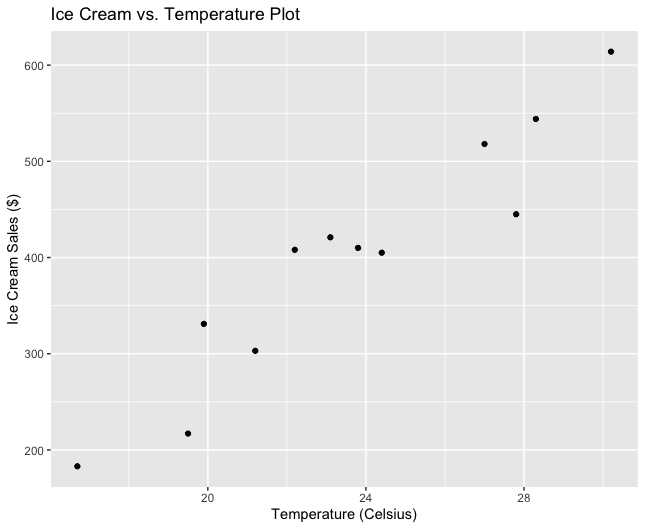
\includegraphics[height=3.5in]{icecream_temp.png}
\end{center}

\begin{center}
    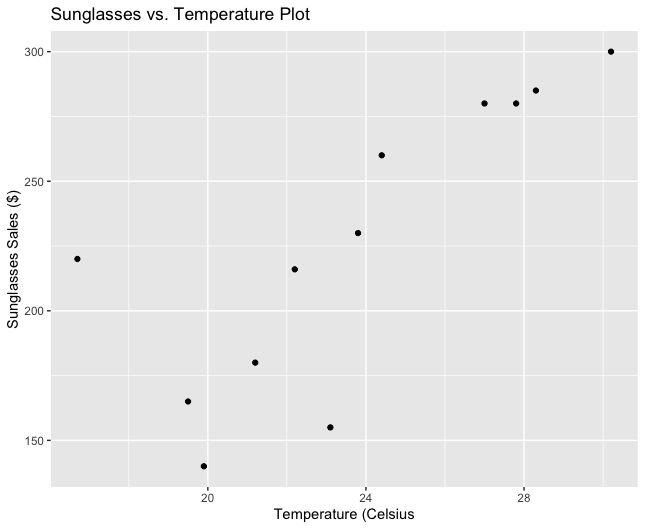
\includegraphics[height=3.5in]{sunglass_temp.png}
\end{center}

\begin{center}
    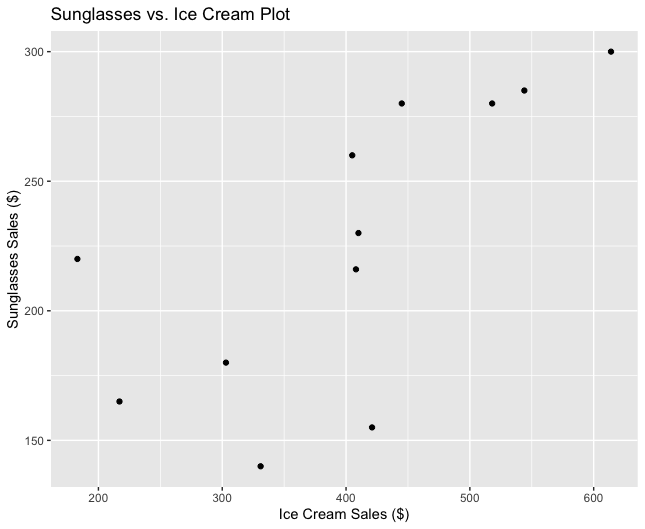
\includegraphics[height=3.5in]{sunglass_icecream.png}
\end{center}

\subsection*{Part B}

No, positive correlation does not mean that one event causes another, just that a certain often happens when another event also happens too, such as buying sunglasses and ice cream.

\newpage

\section*{Question 4}

\subsection*{Part A}

The Central Limit Theorem gives that $L \sim N(n\mu, n\sigma^2)$ so that $P(L \leq X) = \Phi \Big( \frac{X - n\mu}{\sqrt{n}\sigma} \Big)$\\

\noindent Flipping a coin is a Bernouli random variable, so $X \sim Bernouli(.5)$.

$$E(X) = .5 \quad \text{and} \quad Var(X) = p(1-p) = .5(1 - .5) = .25$$

$$P(100X \leq 46) = \Phi \Big( \frac{X - n\mu}{\sqrt{n}\sigma} \Big) = \Phi \Big( \frac{46 - 50}{\sqrt{10} \cdot .5} \Big) = \Phi (-.8) = .212$$

\subsection*{Part B}

$$X \sim Binomial(100, .5)$$

$$P(X \leq 46) = \sum_{i=1}^{46} \binom{100}{i} \cdot .5^i \cdot .5^{100 - i} = \sum_{i=1}^{46} \binom{100}{i} \cdot .5^{100}$$

\begin{lstlisting}[language=R]
     pbinom(46, 100, .5)
\end{lstlisting}

$$P(X \leq 46) = .242$$

\subsection*{Part C}

$$P(100X \leq 46.5) = \Phi \Big( \frac{46.5 - 50}{\sqrt{10} \cdot .5} \Big) = \Phi (-.7) = -.242$$

\newpage

\section*{Question 5}

\subsection*{Part A}

Profit for a house without fire would be \$120 with $P = .99$ while for a house with fire is \$120 minus \$10000 payout, so \$-9880 with $P = .01$.

$$E(X) = .99 \cdot 120 + .01 \cdot -9880 = 20$$

$$E(X_{10}) = 10 \cdot 20 = \$200$$

\subsection*{Part B}

Since there are only 10 houses currently sold insurance, the revenue is \$1200 while the payout for a house with a fire is \$10000 which is significantly more, making any fire a cause of bankruptcy. Since the probability of fire is independent for each house the probability of bankruptcy is:

$$P(fire) = 1 - .99^{10} = .0956$$

\subsection*{Part C}

The Central Limit Theorem gives that $L \sim N(n\mu, n\sigma^2)$ so that $P(L \leq X) = \Phi \Big( \frac{X - n\mu}{\sqrt{n}\sigma} \Big)$\\

\noindent For 1 million homes, the revenue of the company will be \$120000000, so the sum of payouts must be greater than the revenue for bankruptcy, so X will be the payouts.

$$E(X) = .01 \cdot 10000 + .99 \cdot 0 = 100$$

$$Var(X) = E(X^2) - E(X)^2 = .01 \cdot 10000^2 - 100^2 = 990000$$

$$P(X \geq 120000000) = 1 - \Phi \Big( \frac{X - n\mu}{\sqrt{n}\sigma} \Big) = 1 - \Phi \Big( \frac{120000000 - 1000000 \cdot 100}{\sqrt{1000000} \cdot \sqrt{990000}} \Big) = 1 - \Phi (20.1) = 0$$

\noindent Since z score of 20 is very far to the right of the normal distribution.

\newpage

\section*{Question 6}

Light bulb with lifetime exponentially distributed with rate parameter $\lambda = 5$, where L is a random variable for the sum of the lifetimes of 50 independent light bulbs.

\subsection*{Part A}

For one bulb, $L_1 \sim Exp(5)$ so $E(L_1) = 5$ and $Var(L_1) = \frac{1}{25}$.\\

\noindent Since all of the bulbs are independent they sum together:

$$E(L) = \sum^{50} \frac{1}{5} = 50 \cdot \frac{1}{5} = 10$$

$$Var(L) = \sum^{50} \frac{1}{25} = 50 \cdot \frac{1}{25} = 2$$

\subsection*{Part B}

The Central Limit Theorem gives that $L \sim N(n\mu, n\sigma^2)$ so that $P(L \leq X) = \Phi \Big( \frac{X - n\mu}{\sqrt{n}\sigma} \Big)$

$$P(8 \leq L \leq 12) = P(L \leq 12) - P(L \leq 8) = \Phi \Big( \frac{12 - 10}{\sqrt{2}} \Big) - \Phi \Big( \frac{8 - 10}{\sqrt{2}} \Big)$$

$$P(8 \leq L \leq 12) = \Phi (1.41) - \Phi (-1.41) = .9207 - .0793 = .8414$$

\subsection*{Part C}

Interval $(a, b)$ centered on $E(L)$ where $P(a \leq L \leq b) = .95$.\\

\noindent The normal is centered at $E(L)$ so if the contained integral between a and b must be .95 then .05 is left over for the tails of the normal. The probability that L is greater or less than either a or b will be .05 split, so .025.

$$P(E(L) - c \leq .025) = \Phi \Big( \frac{X - n\mu}{\sqrt{n}\sigma} \Big) = \Phi \Big( \frac{10 - c - 10}{\sqrt{2}} \Big) = \Phi \Big( - \frac{c}{\sqrt{2}}\Big)$$

\noindent Based on the standard normal table, a z score of -1.96 will give .025.

$$- \frac{c}{\sqrt{2}} = -1.96 \quad \rightarrow \quad c = 1.96 \cdot \sqrt{2} = 2.77$$

\noindent The interval will then be $(10 - 2.77, 10 + 2.77)$, so that $(a, b) = (7.23, 12.77)$

\end{document}
